\chapter{Fundamentação Teórica}

Este capítulo apresentará a fundamentação teórica desse trabalho de conclusão de curso. Será descrito o estado inicial em que se encontrava o projeto do robô Bellator, com uma visão geral deste ao ser entregue à equipe, a especificação do robô após a reconstrução, a apresentação da Lógica Fuzzy e da metodologia de Mapas Cognitivos Fuzzy (FCM).

%---------- Estado inicial do Projeto ----------
\section{Estado Inicial do Projeto}
\label{chap:estpro}

Esta seção visa descrever com quais recursos a equipe iniciou a execução do trabalho, tanto físicos como lógicos, ou seja, a situação do robô e seus componentes de hardware, o principal recurso material disponível, os componentes de software e a documentação de ambos, da forma como foi entregue à equipe.

\subsection{Visão Geral}

O robô disponibilizado à equipe para a realização desse trabalho, o Bellator, é resultado de um projeto não concluído, visando a implementação de uma plataforma robótica controlada remotamente por joystick. Para tal, o robô foi dividido em três camadas: baixo nível, alto nível e supervisório. A camada de baixo nível seria responsável por controlar os motores do robô, bem como receber leituras dos sensores do mesmo. A camada de alto nível comunicar-se-ia com a camada de baixo nível via conexão serial, faria obtenção de vídeo através de uma webcam e comunicar-se-ia com a camada supervisória através de uma conexão sem fio. Esta última seria a interface com o usuário para realizar o controle remoto do robô. O diagrama esquemático da figura \ref{fig:diagsis} demonstra essa situação.

\begin{figure}[!htb]
	\centering
	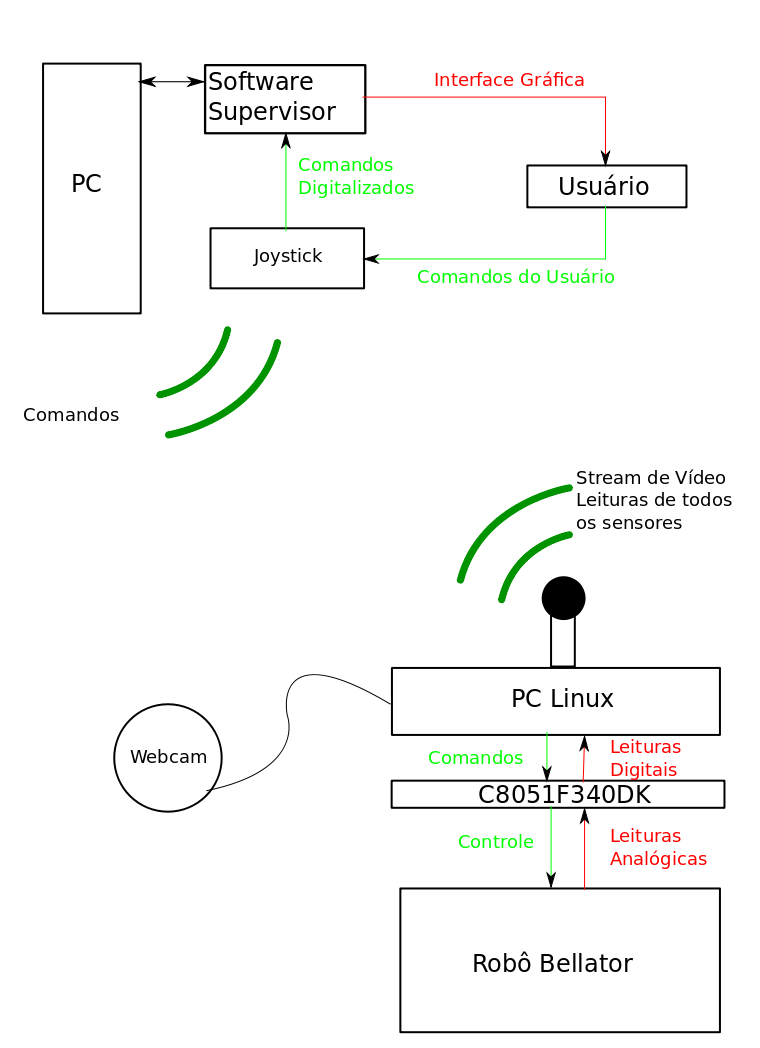
\includegraphics[width=\textwidth]{./figs/diagsis.png}
	\caption[Diagrama original do Bellator]{Diagrama original do projeto Bellator, retirado da monografia do mesmo.}
	\fonte{\cite{BELLATOR}}
	\label{fig:diagsis}
\end{figure}

A partir da figura \ref{fig:diagsis}, o funcionamento do projeto Bellator pode ser explicado. A camada de baixo nível é composta pelo robô Bellator, equipado com dois motores elétricos Bosch FPG 12V, seis sensores de distância "2Y0A02F98" da Sharp, uma bateria Unybatt 12V-7,2 Ampére hora, duas pontes H e a placa microcontrolada C8051F340, capaz de ler e converter leituras de tensão analógicas dos sensores do robô bem como produzir sinais de controle para os motores do robô. Esta placa está conectada à camada de alto nível, composta por um PC Embarcado VIA EPIA ME60000 Mini-ITX com sistema operacional Linux, através de uma conexão serial. Utilizando-se de um protocolo de comunicação, esse PC embarcado envia comandos de movimentação para a camada de baixo nível e recebe as leituras dos sensores obtidas pela camada de baixo nível. O PC embarcado também comunica-se com a camada de alto nível para receber comandos de movimentação do usuário e enviar as leituras dos sensores para o mesmo. Além disso, o PC embarcado envia, também via comunicação sem fio, um stream de vídeo gerado por uma webcam Genius iLook 316. Finalmente, o software supervisor remoto, executado em um PC com máquina virtual Java, fornece as informações recebidas da camada de alto nível para o usuário, permitindo-o tomar decisões sobre a locomoção do robô. O software também recebe comandos de movimentação do usuário, gerados em um Joystick do videogame Sony Playstation 2, enviando-os para a camada de alto nível pela mesma conexão.

O leitor pode observar que o projeto Bellator apresenta objetivos muito distintos do projeto "Algoritmos de Navegação Fuzzy: Uma Análise Qualitativa". Assim, não será feita uma descrição detalhada de todos os componentes do projeto Bellator. A seguir, será descrito como o robô foi recebido pela equipe e quais componentes foram reaproveitados.

\subsection{Recebimento do Robô}
\label{sec:recrobo}

O robô Bellator foi entregue à equipe em Abril de 2011, em uma caixa, desmontado, juntamente com toda a documentação disponível por mídia digital. A caixa continha os seguintes itens:

\begin{itemize}
\item Chassi do robô Bellator com dois motores Bosch FPG12V e pontes H acoplados;
\item Cinco sensores de distância "2Y0A02F98" da Sharp;
\item Duas baterias Unybatt 12V-7,2 Ampére hora;
\item Uma placa micro-controlada C8051F340;
\item Uma placa de roteamento, produzida pelo projeto Bellator;
\item Um PC Embarcado VIA EPIA ME60000 Mini-ITX.
\end{itemize}

O chassi do robô e seus componentes acoplados são a base da plataforma robótica a ser utilizada pela equipe e são críticas para a execução desse trabalho. Os sensores de distância, um a menos que os disponíveis no projeto Bellator, são essenciais para a localização do robô e de obstáculos. A placa microcontrolada também é um recurso crítico, pois é o componente responsável por todo o controle de baixo nível do robô cujo software e a documentação serão reaproveitados do projeto Bellator. As baterias são um recurso necessário e de fácil aquisição, ao contrário dos outros componentes citados.

Alguns itens mencionados na seção anterior, referentes ao projeto Bellator, não foram recebidos ou não serão utilizados nesse trabalho. A webcam e joystick não foram entregues pois não serão necessários, visto que um sistema de navegação autônomo não necessita de joystick e esse trabalho não abordará navegação através de imagem de vídeo. A placa de roteamento entregue será utilizada nos testes dos componentes, visto que é essencial para o funcionamento do robô. Esta placa será reprojetada e reconstruída. O PC embarcado foi entregue destituído de qualquer documentação. Além disso, como o novo objetivo do robô não necessita de comunicação semfio e não utilizará stream de vídeo, motivo principal para a utilização deste PC no projeto anterior, a equipe optou por descartar este recurso do projeto e utilizar outra placa mais simples e menor, que será descrita em detalhes na seção \ref{chap:esprob}.

A documentação disponível à equipe, produzida durante o projeto Bellator, descreve em detalhes os componentes de hardware dessa plataforma robótica, o software de controle supervisório e a camada de baixo nível, ou seja, o software da placa C8051F340\cite{BELLATOR}. Essa documentação será utilizada como referência para o reaproveitamento do projeto Bellator nesse trabalho, com exceção da documentação referente ao software de controle supervisório, que não será utilizado.

\subsection{Considerações}
A possibilidade de reaproveitamento parcial do projeto Bellator e o recebimento desse material consistiram uma importante epata nesse trabalho. A plataforma Bellator é uma opção de recurso ao apoio do estudo qualitativo proposto nesse TCC.

%---------- Especifica��es do hardware do rob� ----------
\section{Especifica��es do Rob�}
\label{sec:esprob}

Esta se��o visa descrever a composi��o de \emph{hardware} do rob�
Bellator ap�s a reconstru��o e adequa��o do mesmo. Essa decri��o
inclui a apresenta��o dos sensores infravermelhos, enconders
�pticos, placa microcontrolada C8051F340DK, placa TS-7260, placa de roteamento e a apresenta��o do produto final, ou seja, o rob� montado.

\subsection{Sensor IR 2Y0A02F98}
\label{sec:sensores}
O sensor 2Y0A02F98 � um sensor anal�gico infravermelho e mede dist�ncias no intervalo de 20 a 150 cent�metros \cite{datasheetsensor}, sendo que os valores de tens�o de resposta do sensor seguem a curva mostrada na figura \ref{curva}. Como o valor de leitura � anal�gico, foi necess�rio que a placa C8051F340DK fosse programada para converter essa leitura em digital. O c�digo de convers�o est� de acordo com o projeto Bellator \cite{BELLATOR} e tamb�m efetua a transfer�ncia desses dados por comunica��o serial.

\begin{figure}[H]
  \centering
  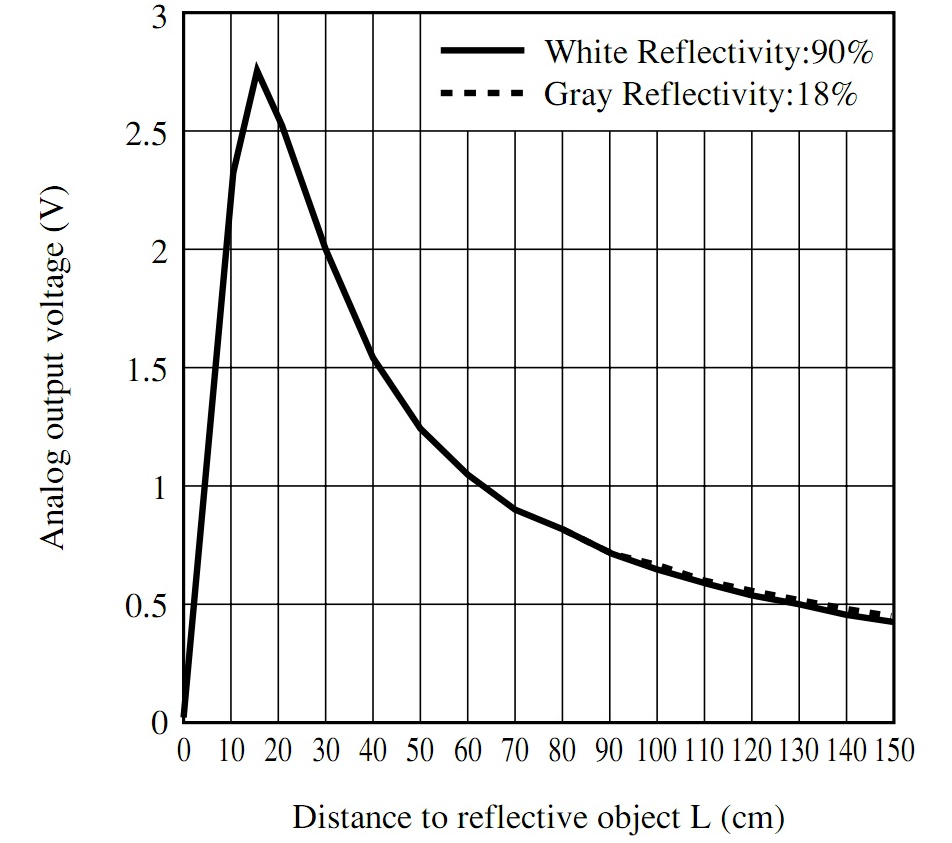
\includegraphics[width=0.5\textwidth]{./figs/curvaresp.png}
  \caption[Curva de resposta do sensor de dist�ncia]{Curva de resposta do sensor de dist�ncia.}
  \fonte{\cite{datasheetsensor}}
  \label{curva}
\end{figure}

O modelo � pouco influenciado pelas cores dos objetos refletidos, isso � devido ao m�todo de medi��o baseado em triangula��o \cite{datasheetsensor}. O sensor possui uma tens�o de alimenta��o recomendada na faixa de 4,5 a 5,5 V \cite{datasheetkit}. Como as baterias dispon�veis eram de 12 V, foi necess�ria utiliza��o de um regulador de tens�o. O c�lculo dos valores dos resistores foram baseados na equa��o \ref{eqRegulador} e o diagrama esquem�tico do regulador � mostrado na figura \ref{regulador}. Esse circuito comp�e uma das partes da placa de roteamento, conforme mostrado na se��o \ref{sec:espplacaroteamento}.

\begin{equation}
\label{eqRegulador}
V_{OUT} = 1,25V (1 + R_{2}/R_{1})
\end{equation}

\begin{figure}[H]
  \centering
  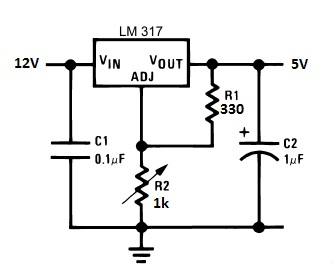
\includegraphics[width=0.5\textwidth]{./figs/regulador.jpg}
  \caption[Diagrama esquem�tico do regulador de tens�o dos sensores de dist�ncia]{Diagrama esquem�tico do regulador de tens�o dos sensores de dist�ncia.}
  \fonte{\cite{LM317}}
  \label{regulador}
\end{figure}

O modelo em quest�o � adequado ao projeto pois apresenta dimens�es compat�veis com o chassi do rob� e, como a finalidade desses sensores � auxiliar a navega��o do rob� em ambientes fechados, a faixa de resposta � suficiente para detec��o de objetos. Contudo, h� a possibilidade de, em projetos futuros, acrescentar outros tipos de sensores mais precisos voltados � medi��o de dist�ncias menores.

\subsection{Encoder �ptico HEDS-9700}
\label{sec:heds9700}
O \emph{encoder} �ptico HEDS-9700 � um circuito capaz de gerar uma onda quadrada � medida que um \emph{encoder} de quadratura � rotacionado \cite{HEDS9700}. A curva de resposta desse sensor � ilustrada na figura \ref{fig:HEDS-9700}. Nessa figura s�o ilustrados dois canais A e B, havendo um defasamento de $\phi$ entre os sinais. Nesse projeto, foi utilizado o sinal de apenas um dos canais, pois a informa��o desejada era simplesmente a contagem de pulsos gerada por cada encoder. O \emph{encoder} de quadratura utilizado na plataforma rob�tica est� fixado no eixo de cada roda e apresenta 1800 pulsos por volta. A placa C8051F340DK foi programada para contar esses pulsos e fornecer uma medida odom�trica para realimenta��o da velocidade. Essa programa��o � descrita na se��o \ref{sec:codmicro} e permite ajustar a velocidade das rodas de forma independente. Como a placa de roteamento do projeto de oficinas \cite{BELLATOR} n�o foi projetada para tratar o sinal deste \emph{encoder}, foi projetada uma nova vers�o dessa placa, descrita na se��o \ref{sec:espplacaroteamento}.

\begin{figure}[H]
  \centering
  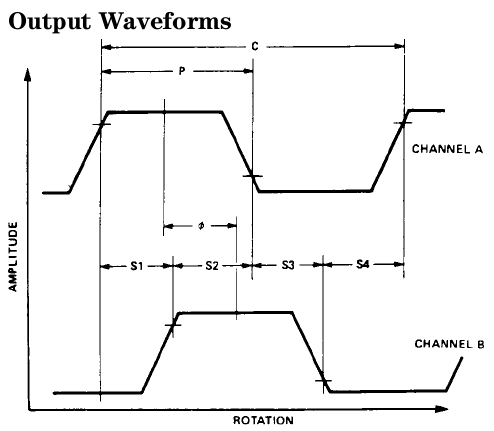
\includegraphics[width=0.5\textwidth]{./figs/HEDS-9700.png}
  \caption[Formas de onda de sa�da do \emph{encoder} �ptico]{Formas de onda de sa�da do encoder �ptico.}
  \label{fig:HEDS-9700}
  \fonte{\cite{HEDS9700}}
\end{figure}

\subsection{C8051F340DK}
\label{sec:C8051F340DK}

O C8051F340 � uma unidade microcontroladora (MCU) equipada com um n�cleo da fam�lia 8051 e v�rios dispositivos perif�ricos dispostos em uma placa de circuito impresso. As especifica��es dessa unidade foram retiradas do relat�rio do projeto Bellator \cite{BELLATOR}. O diagrama em blocos do kit � apresentado na figura \ref{dbloc}. A C8051F340 possui as seguintes caracter�sticas \cite{datasheetkit}:

\begin{itemize}
  \item Conversor ADC 10 bits de at� 200 ksps (amostras por segundo);
  \item Dois comparadores;
  \item \emph{Brown-out Reset} e \emph{Power-on Reset};
  \item Tens�o de Refer�ncia interna;
  \item Porta USB 2.0;
  \item Duas \emph{interfaces} seriais (UART) e uma \emph{interface} SPI;
  \item Fonte de Alimenta��o de 2.7 at� 5.25V regulada internamente;
  \item Micro-processador 8051 de at� 48 MIPS;
  \item 4352 Bytes de mem�ria RAM;
  \item 40 Portas de E/S;
  \item 4 temporizadores de 16 bits;
  \item Sele��o de \emph{clock} interno de alta ou baixa velocidade ou \emph{clock} externo.
\end{itemize}

\begin{figure}[H]
  \centering
  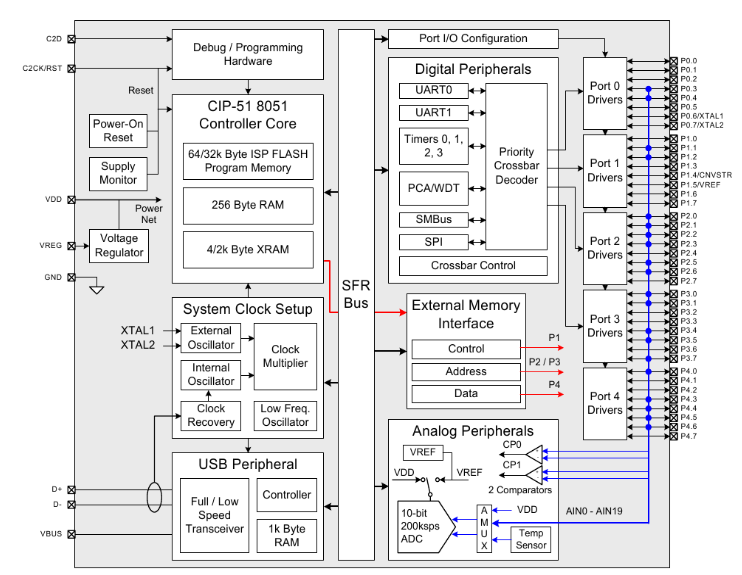
\includegraphics[width=0.8\textwidth]{./figs/dbloc.png}
  \caption[Diagrama em blocos do kit C8051F340DK]{Diagrama em blocos do kit C8051F340DK.}
  \fonte{\cite{datasheetkit}}
  \label{dbloc}
\end{figure}

\subsection{Placa TS-7260}
\label{sec:espts7260}

A placa TS-7260 � um sistema embarcado equipado com um processador ARM e sistema operacional Linux. O sistema possui perif�ricos para realiza��o de comunica��o serial, ethernet, usb, entre outros. A lista a seguir descreve os componentes relevantes para o projeto. Os dados, bem como a figura \ref{fotots}, foram retirados do \emph{datasheet} \cite{TS-7260}.

\begin{itemize}
  \item Processador ARM9 de 200MHz baseado no Cirrus EP9302
  \item 32MB de mem�ria NAND Flash
  \item 32MB de mem�ria SDRAM
  \item Consumo menor que 1 Watt mesmo em capacidade m�xima
  \item Porta Ethernet 10/100
  \item Duas portas USB 2.0
  \item Entrada de 4.5 a 20 Volts
  \item Dimens�es: 9.7 cm por 11.5cm
\end{itemize}

\begin{figure}[H]
  \centering
  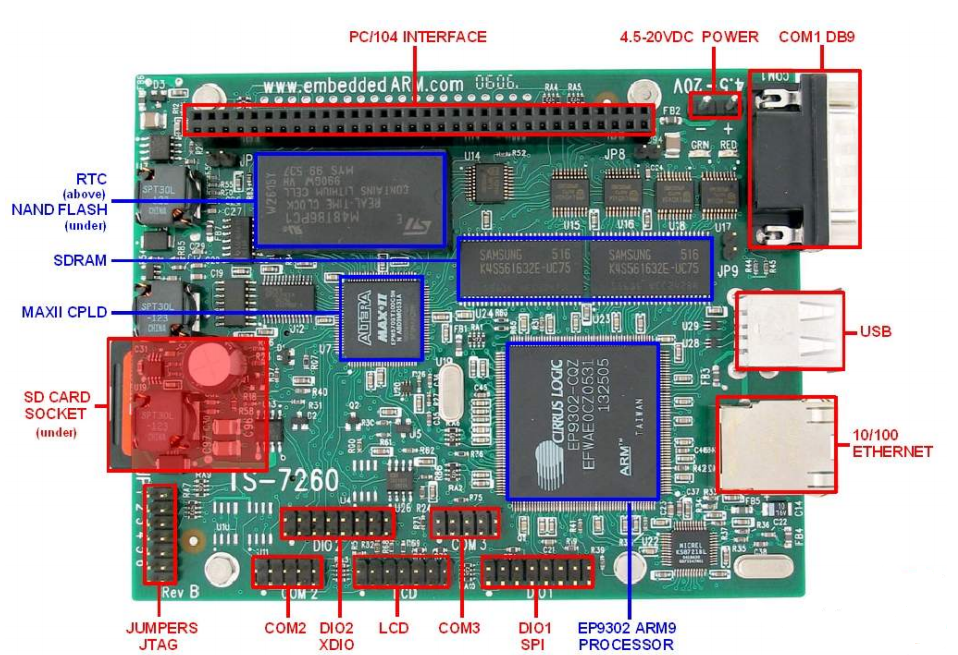
\includegraphics[width=0.8\textwidth]{./figs/fotots.png}
  \caption[Foto da placa TS-7260]{Foto da placa TS-7260.}
  \fonte{\cite{tsmanual}}
  \label{fotots}
\end{figure}

Mais informa��es sobre o sistema, bem como a documenta��o completa, est�o dispon�veis no manual da placa, dispon�vel nas refer�ncias bibliogr�ficas \cite{tsmanual}.

\subsection{Placa de Roteamento}
\label{sec:espplacaroteamento}

A placa de roteamento � um componente desenvolvido com base na placa dispon�vel do projeto Bellator \cite{BELLATOR}. Como a placa de roteamento recebida com o Bellator n�o tratava os sinais dos \emph{encoders} e estava constru�da de forma rudimentar, em uma placa universal, ela foi reprojetada e reconstru�da pela equipe. As especifica��es da placa de roteamento s�o:
\begin{itemize}
    \item Dimens�es: 5 x 9 cm;
    \item Trilhas de cobre de aproximadamente 1 mm;
    \item Regulador de tens�o LM317T: Entrada at� 40V, Sa�da 5,05V;
    \item \emph{Buffer} para PWM: 74LS244;
    \item Conectores para cabos \emph{flat}, PWM, Sensores e \emph{Encoders}.
\end{itemize}

O projeto da placa, m�todos de desenvolvimento, requisitos, entre outros ser�o descritos de forma detalhada na se��o \ref{sec:desroteamento}.

\subsection{Rob� Bellator}
\label{sec:robobellator}

O rob� Bellator, como mencionado na se��o \ref{sec:estpro}, foi reconstru�do e adaptado ao projeto. O rob� consiste de um chassi de 40 cm de largura por 50 cm de comprimento, duas rodas de tra��o e uma roda guia, conforme ilustrado na figura \ref{fig:dispsensor}. As rodas de tra��o est�o nas laterais da parte dianteira do rob� e possuem di�metro de 20 cm e largura de 4 cm. Ambas possuem o \emph{encoder} �ptico HEDS-9700, descrito na se��o \ref{sec:heds9700}, fixados nos respectivos eixos. A roda guia est� no centro da parte traseira do rob� e possui di�metro de aproximadamente 6 cent�metros e espessura de 2 cent�metros. Todas as rodas s�o da marca Schioppa e chassi do rob� permanece a 3 cm da superf�cie do solo. Com o objetivo de auxiliar a navega��o do rob� e fazer varreduras do ambiente, foram fixados cinco sensores do modelo 2Y0A02F98, descrito na se��o \ref{sec:sensores}, dispostos uniformemente nas laterais do chassi, conforme ilustra a figura \ref{fig:dispsensor}. Os outros componentes do rob� est�o listados a seguir:
\begin{itemize}
  \item[-] 2 Motores Bosch FPG 12V;
  \item[-] 2 Baterias Unybatt 12V-7,2 Amp�re-hora;
  \item[-] Duas pontes H L 298.
\end{itemize}

\begin{figure}[H]
  \centering
  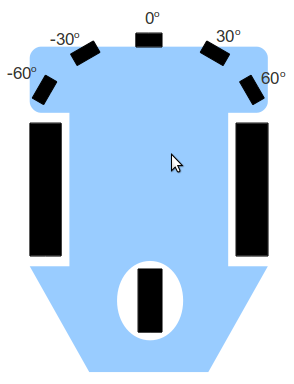
\includegraphics[width=0.3\textwidth]{./figs/dispsensor.png}
  \caption[Disposi��o dos sensores infravermelhos e rodas]{Disposi��o dos sensores infravermelhos e rodas.}
  \fonte{Autoria pr�pria}
  \label{fig:dispsensor}
\end{figure}

A plataforma transporta as placas do sistema microcontrolado C8051F340DK, descrito na se��o \ref{sec:C8051F340DK}, o sistema embarcado TS-7260, descrito na se��o \ref{sec:espts7260} e a placa de roteamento, descrita na se��o \ref{sec:espplacaroteamento}. O rob� montado pode ser visualizado na figura \ref{bellator}, que ilustra a disposi��o dos sensores infravermelhos, rodas, baterias e placas no chassi.

\begin{figure}[H]
  \centering
  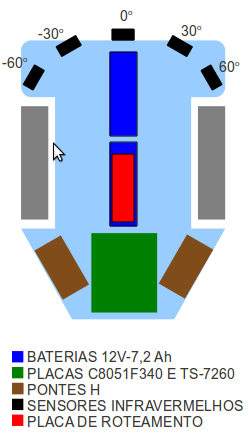
\includegraphics[width=0.3\textwidth]{./figs/bellator.png}
  \caption[Rob� Bellator montado]{Rob� Bellator montado.}
  \fonte{Autoria pr�pria}
  \label{bellator}
\end{figure}



\section{Lógica Fuzzy}
Essa seção tem como função descrever o que é a lógica fuzzy, como surgiu, como funciona e como projetar um sistema fuzzy.

A lógica fuzzy é baseada no trabalho de Lofti Zadeh, que propôs a teoria de conjuntos
fuzzy em 1965~\cite{FUZZYLOGIC}. Na teoria clássica de conjuntos, um elemento tem seu
grau de pertinência ao conjunto representado por uma variável booleana, ou seja, ou o elemento
pertence ao conjunto ou não pertence. Num conjunto fuzzy, no entanto, um elemento tem seu grau
de pertinência representado por um valor real no intervalo [0, 1].

Uma aplicaçao básica e clássica da lógica fuzzy é a classificação de uma variável contínua. Por exemplo,
para classificar um valor de temperatura, pode-se utilizadar um conjunto fuzzy com as variáveis
FRIO, MORNO e QUENTE. Para classificar dado valor de temperatura, pode se utilizar as classes fuzzy apresentadas
 na figura \ref{fig:fuzzyclasses}.

\begin{figure}[!htb]
    \centering
    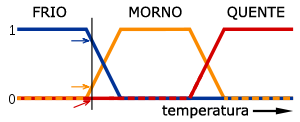
\includegraphics{./figs/fuzzyclasses.png}
    \caption[Classificação Fuzzy]{Classificação de valores de temperatura utilizando lógica fuzzy.}
    \fonte{\cite{FUZZYLOGIC}}
    \label{fig:fuzzyclasses}
\end{figure}

A temperatura destacada na figura tem os seguintes graus de pertinência: 0.8 FRIO, 0.2 MORNO e 0 QUENTE.
É comum também associar outras variáveis linguísticas para caracterizar os valores. No caso do exemplo, uma associação
possível seria: bastante frio, levemente morno, nada quente.

Com base na saída do classificador, um sistema fuzzy pode realizar inferências. Por exemplo, caso o objetivo fosse controlar
a temperatura de uma caldeira, visando deixá-la bem quente, a observação de que está bastante frio implicaria
na necessidade da elevação da quantidade de energia disponibilizada para seu aquecimento. Conforme a temperatura aumenta, novas temperaturas seriam observadas e classificadas em graus menores de frio e maiores de morno ou quente. Estas novas classificações levam a inferências diferentes e a outras alterações na fonte de calor, até alcançar a temperatura esperada. Quanto mais próximo do nível esperado, menos calor deverá ser suprido pela fonte de calor para o sistema, neste exemplo.

As decisões tomadas pelo sistema são definidas por um conjunto de regras fuzzy, cujo formato básico é:

SE X ENTÃO Y

onde X é uma expressão contendo uma ou mais variáveis linguísticas e Y a ação a ser tomada. Retomando o exemplo da caldeira,
uma regra possível seria: SE bastante frio ENTÃO aumentar bastante o fornecimento de calor.

É evidente que os conceitos FRIO, MORNO e QUENTE são totalmente subjetivos e cada aplicação tem parâmetros e conceitos específicos, em variáveis linguísticas diferentes, tais como velocidade, distância, pressão, entre outros.
Os valores e funções utilizadas para classificar tais grandezas são determinados por quem está desenvolvendo o sistema fuzzy, com os devidos ajustes para melhor adequação à aplicação em questão. 
Da mesma forma, as decisões a serem tomadas com base nos dados classificados são definidas pelo desenvolvedor. A grande vantagem e, até mesmo, objetivo de um sistema fuzzy é proporcionar um raciocínio simples na implementação das regras de um sistema. Isso é
interessante quando se considera a adição de novos sensores e, consequentemente, novos dados. Uma simples alteração ou adição
de novas regras é o suficiente para adaptar o sistema às novas entradas. %Não é verdade, necessariamente? Novos dados/entradas -> Muitas novas regras.

Pelo fato de permitir a classificação de dados de uma forma mais flexível, em comparação com a teoria clássica de conjuntos,
os dados de entrada para um sistema fuzzy não precisam ser tão precisos, sem ruídos, já que a presença de ruídos
causa apenas pequenas variações na classificação, enquanto numa classificação binária, pouco ruído pode
ocasionar a passagem de um nível baixo para um nível alto subitamente, ao passar um limite pré-definido.

Para projetar um sistema fuzzy, o seguinte conjunto de passos pode ser seguido \cite{FUZZYLOGICTUTORIAL}:

\begin{enumerate}
    \item Definição do que vai ser controlado, com quais critérios, qual o tipo de saída desejado;
    \item Determinação da relação entre a entrada e a saída, escolha do número de variáveis de entrada para o sistema;
    \item Utilizando a estrutura de regras da lógica fuzzy, dividir o problema principal em várias tarefas menores. Estas
    regras devem descrever o comportamento desejado conforme definido no item 1. O número e complexidade das regras depende do número de parâmetros de entrada a serem processados e do número de variáveis fuzzy associadas aos mesmos;
    \item Criação das funções de classificação, que definem os significados (comumente através de variáveis linguísticas);
    dos valores de entrada e saída. As saídas das funções de classificação serão utilizadas nas regras
    \item Criação das funções para pré e pós-processamento necessárias (para tratamento dos dados de entrada e saída);
    \item Testar o sistema, avaliar os resultados, ajustar as regras e funções de classificação. Repetir este passo;
    até obter um comportamento satisfatório.
\end{enumerate}

\subsection{Considerações}

O conceito de incerteza introduzido pela Lógica Fuzzy permite a modelagem de sistemas problemas de decisão cujas variáveis são dinâmicas e admitem vários níveis de classificação. O problema de navegação robótica
é um sistema dinâmico, pois as decisões são tomadas sob a influência de vários sensores ao mesmo tempo, e a abordagem Fuzzy é uma opção para solucioná-lo.

\section{Mapas Cognitivos Fuzzy}

Esta seção tem como objetivo explicar o que são mapas cognitivos fuzzy, também conhecidos como FCM (Fuzzy Cognitive Maps), abordando o conceito, a estrutura, as propriedades e vantagens desse modelo, apresentar os passos para contrução de um FCM e apresentar exemplos, que descrevem o uso em situações reais.

O modelo FCM é abordado na tese de doutorado de \cite{FCMENDONCA}. Mapas cognitivos são diagramas que representam ligações entre palavras, idéias, tarefas ou outros itens ligados a um conceito central, dispostos radialmente, intuitivamente e de acordo com a importância de cada conceito. Crenças ou afirmações a respeito de um domínio de conhecimento limitado são expressas por palavras ou expressões linguísticas interligadas por relações de causa e efeito, que possibilitam predizer as consequências que essa organização implica ao universo representado. O mapa cognitivo fuzzy é gerado quando se incluem a essa estrutura incertezas através da lógica Fuzzy.

A estrutura de um FCM é um grafo direcionado, figura \ref{fig:fcm}, em que os valores numéricos são variáveis ou conjuntos fuzzy, os "nós" são conceitos linguísticos, representados por conjuntos fuzzy e cada "nó" é associado a outros nós através de conexões, a cada qual está associado um peso numérico, que representa a variável fuzzy relacionada ao nível de causalidade entre os conceitos. Um mapa cognitivo fuzzy descreve um sistema em termos de conceitos, onde cada conceito representa uma entidade, um estado, uma variável ou uma característica do sistema. Os conceitos (C1 a C5) podem ser atualizados através da interação com outros conceitos por meio das relações causais (wi,j) e com seu próprio valor. A matriz \ref{fcm-matrix} representa o peso das relações causais entre os conceitos e podem ser atualizados através da equação \ref{fcm-update}. Esta descreve a evolução do FCM, na qual j é o contador das iterações, n é o número de nós do grafo, Wij é o peso do arco que conecta o conceito Cj ao conceito Ci, Ai e Ai_anterior são o valor do conceito Ci na iteração atual e anterior, respectivamente, e a função f \ref{sigmoide} é uma função do tipo sigmóide.

\begin{figure}[!htb]
    \centering
    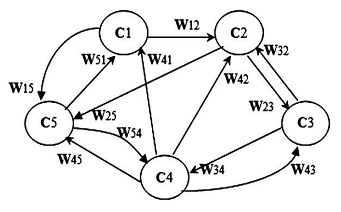
\includegraphics{./figs/fcm.png}
    \caption[Mapa Cognitivo Fuzzy]{Exemplo de um FCM (grafo).}
    \fonte{\cite{FCMENDONCA}}
    \label{fig:fcm}
\end{figure}

\begin{equation}\label{fcm-matrix}
    wi,j=\left(
       \begin{array}{ccccc}
         0 & w12 & 0 & 0 & w15 \\
         0 & 0 & w23 & 0 & w25 \\
         0 & w32 & 0 & w34 & 0 \\
         w41 & 0 & w43 & 0 & w45 \\
         w51 & 0 & 0 & w54 & 0 \\
       \end{array}
     \right)
\end{equation}

\begin{equation}\label{fcm-update}
Ai=f(sum{AjxWji})+Ai
\end{equation}

\begin{equation}\label{sigmoide}
f(x)={1}/{1+e^-lx}
\end{equation}

Um FCM apresenta as propriedade de elasticidade e estabilidade. A elasticidade, ou auto organização, é a capacidade de reforçar ou enfraquecer o peso das relações causais entre os conceitos e a estabilidade é a capacidade de evoluir, estabilizando-se em um ponto fixo ou após um número máximo de iterações. Uma vantagem do FCM é a modularidade, a qual permite que um problema complexo seja representado por vários mapas modulares e outra vantagem é a que os pesos das relações causais e dos conceitos podem ser obtidos via treinamento a partir dos dados históricos do sistema ou através de um algoritmo adaptativo, que atualiza os pesos constantemente.

Na tese de \cite{FCMENDONCA}, são apresentados os seguintes passos para construção de um FCM:

\begin{itemize}{*}{}
\item Passo 1 – Identificação dos conceitos e das suas interconexões ou relações
determinando a natureza (positiva, negativa, neutra) das relações causais entre
conceitos.
\item Passo 2 – Aquisição de dados iniciais, através de ponderação de opinião de
especialistas e ou análise do sistema de equações, quando se conhece o modelo
matemático.
\item Passo 3 – Apresentação dos dados referentes à opinião dos diversos especialistas a
um sistema lógico fuzzy que tem como saída os valores dos pesos do FCM.
\item Passo 4 – Tratamento da informação, adaptação e ou otimização do FCM
inicialmente proposto, ajustando suas respostas às saídas desejadas.
\item Passo 5 – Validação do FCM ajustado nas condições de operação do sistema ou
processo modelado.
\end{itemize}

Em \cite{FCMENDONCA} os mapas cognitivos fuzzy são aplicados no controle de processos industriais. Um exemplo de aplicação é mostrado na figura \ref{fig:fcm-exemplo-planta}, na qual é ilustrado um tanque com duas válvulas de entrada (V1 e V2) para diferentes tipos de líquidos, um misturador, uma válvula de saída (V3) para o líquido misturado e um medidor de massa específica (G) que mede a quantidade de líquido produzida. As válvulas V1 e V2 introduzem dois líquidos diferentes. Durante a mistura, o medidor de massa específica verifica quando o produto atingiu o ponto adequado e, desse modo, a válvula V3 é ativada e o produto da mistura é esvaziado. Com isso, o controle do processo é manter as variáveis V e G, sendo V o volume e G a massa especifica do produto no tanque, dentro das faixas de operação [Vmin, Vmax] (equação \ref{lim-V}) e [Gmin, Gmax] (equação \ref{lim-G}), respectivamente. Analisando-se o problema, os seguintes conceitos podem ser definidos.

\begin{figure}[!htb]
    \centering
    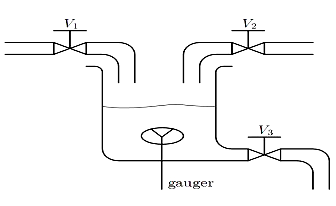
\includegraphics{./figs/fcm-exemplo-planta.png}
    \caption[Mapa Cognitivo Fuzzy]{Aplicação do FCM em processo industrial.}
    \fonte{\cite{FCMENDONCA}}
    \label{fig:fcm-exemplo-planta}
\end{figure}

\begin{equation}\label{lim-V}
Vmin<V<Vmax
\end{equation}

\begin{equation}\label{lim-G}
Gmin<G<Gmax
\end{equation}

\begin{itemize}
\item Conceito 1: Volume de líquido no tanque, o qual depende do estado das válvulas V1, V2 e V3;
\item Conceito 2: Estado da válvula 1 (fechada, aberta ou parcialmente aberta);
\item Conceito 3: Estado da válvula 2 (fechada, aberta ou parcialmente aberta);
\item Conceito 4: Estado da válvula 3 (fechada, aberta ou parcialmente aberta);
\item Conceito 5: Valor de massa específica do líquido medido pelo sensor G.
\end{itemize}

Interligando-se os conceitos com as relações de causa e efeito, obtém-se o FCM da figura \ref{fig:fcm-exemplo-fcm} para o controlador do processo. Além dos conceitos, os especilistas no processo determinaram um domínio para as variáveis que resultou em uma faixa de valores para as relações causais, equações \ref{peso-1} a \ref{peso-8}. Após a estabilização do mapa, obteve-se os pesos da matrix \ref{W-matrix} e os valores dos conceitos da matrix \ref{A-matrix} e, desse modo, os limites das equações \ref{lim-V} e \ref{lim-G} são reajustados para os valores correspondentes às equações \ref{lim-V-adj} e \ref{lim-G-adj}, respectivamente.

\begin{equation}\label{peso-1}
-0,50<W12<0,30
\end{equation}
\begin{equation}\label{peso-2}
-0,40<W13<0,20
\end{equation}
\begin{equation}\label{peso-3}
0,20<W15<0,40
\end{equation}
\begin{equation}\label{peso-4}
0,30<W21<0,40
\end{equation}
\begin{equation}\label{peso-5}
0,40>W31<0,50
\end{equation}
\begin{equation}\label{peso-6}
-1,0<W41<0,80
\end{equation}
\begin{equation}\label{peso-7}
0,50<W52<0,70
\end{equation}
\begin{equation}\label{peso-8}
0,30<W54<0,40
\end{equation}

\begin{figure}[!htb]
    \centering
    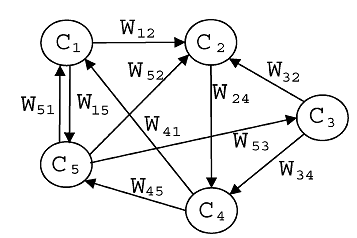
\includegraphics{./figs/fcm-exemplo-fcm.png}
    \caption[Mapa Cognitivo Fuzzy]{FCM do controlador.}
    \fonte{\cite{FCMENDONCA}}
    \label{fig:fcm-exemplo-fcm}
\end{figure}

\begin{equation}\label{W-matrix}
    Winicial=\left(
       \begin{array}{ccccc}
         0,00 & -0,40 & -0,25 & 0,00 & 0,30 \\
         0,36 & 0,00 & 0,00 & 0,00 & w0,00 \\
         0,45 & 0,00 & 0,00 & 0,00 & 0,00 \\
         -0,90 & 0,00 & 0,00 & 0,00 & 0,00 \\
         0,00 & 0,60 & 0,00 & 0,30 & 0,00 \\
       \end{array}
     \right)
\end{equation}

\begin{equation}\label{A-matrix}
    Winicial=\left(
       \begin{array}{ccccc}
         0,10 & 0,45 & 0,39 & 0,04 & 0,01 \\
       \end{array}
     \right)
\end{equation}

\begin{equation}\label{lim-V-adj}
0,68<V<0,70
\end{equation}

\begin{equation}\label{lim-G-adj}
0,78<G<0,85
\end{equation}

Outra aplicação é descrita no artigo \cite{MENDONCA}, na qual a abordagem FCM é empregada em navegação robótica. Nesse artigo, um modelo de FCM novo é implementado para suportar as condições dinâmicas dos sistemas de navegação, nas quais os valores das relações causais são modificados dinamicamente através da ocorrência de eventos especiais. Os autores do artigo chamaram esse modelo de ED-FCM (Event-Driven Fuzzy Cognitive Map). O ajuste dos pesos das relações causais é efetuado por um algoritmo de aprendizado por reforço, conforme ilustra a figura \ref{fig:reinforcement-alg}, e permite que o robô (agente) aprenda diretamente através de sua interação com o ambiente. A cada instante de tempo t, o agente estabelece, por meio de seus sensores, um estado st e, de acordo com suas regras, determina uma ação at a ser efetuada pelos atuadores. Essa ação causa uma transição para o estado st+1 e o ambiente retorna uma medida de reforço rt+1, que pode ser uma recompensa (caso a ação seja boa) ou uma punição (caso a ação seja ruim).

\begin{figure}[!htb]
    \centering
    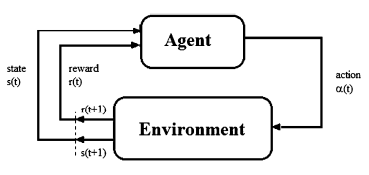
\includegraphics{./figs/reinforcement.png}
    \caption[Mapa Cognitivo Fuzzy]{Algoritmo de aprendizado por reforço.}
    \fonte{\cite{MENDONCA}}
    \label{fig:reinforcement-alg}
\end{figure}

Primeiramente, foi construído um FCM que descreve o comportamente reativo do robô, no qual a leitura dos sensores de distância (esquerdo, frontal e direito) levam a uma ação imediata que interfere no movimento do robô. Os seguintes conceitos foram definidos e o FCM da figura \ref{fcm-robot} foi projetado.

\begin{itemize}
\item Conceito R.S.: Leitura do sensor da direita;
\item Conceito F.S.: Leitura do sensor frontal;
\item Conceito L.S.: Leitura do sensor esquerdo;
\item Conceito L.O.: Representa decisões sobre virar a esquerda;
\item Conceito R.O.: Representa decisões sobre virar a direita;
\item Conceito L.O.(-1): Decisão anterior sobre virar a esquerda;
\item Conceito R.O.(-1): Decisão anterior sobre virar a direita;
\item Conceito Out Left: O robô vira à esquerda;
\item Conceito Out Front: O robô acelera;
\item Conceito Out Right: O robô vira à direita.
\end{itemize}

\begin{figure}[!htb]
    \centering
    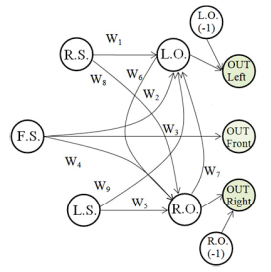
\includegraphics{./figs/fcm-robot.png}
    \caption[Mapa Cognitivo Fuzzy]{FCM do comportamento reativo do robô.}
    \fonte{\cite{MENDONCA}}
    \label{fig:fcm-robot}
\end{figure}

\subsection{Considerações}
FCM é um modelo linguístico, próximo à linguagem humana, que é baseado na teoria de grafos e que permite interconectar conceitos através de relações de causa e efeito ponderadas. Essa abordagem apresenta a vantagem da modularidade, que possibilita dividir um problema complexo em diversos submodelos. Um FCM introduz a incerteza Fuzzy e tem a capacidade de integração com métodos de treinamento de inteligência artificial. O FCM é indicado para modelagem de sistemas complexos. A navegação robótica é um sistema complexo no qual vários conceitos (sensores e motores) são ativados e interagem entre si para produzir os movimentos adequados ao robô autônomo. A abordagem FCM permite modelar e mapear esses conceitos com a finalidade de implementar um algoritmo de navegação capaz de solucionar o problema.

